\section{Silicon energy bands}

\addtolength{\hoffset}{-1.5cm}
\begin{small}
\begin{center}
\begin{longtable}{|c|c|c|c|c|}

% Header for first page
\hline 
\multicolumn{1}{|c|}{\textbf{Energy}} & 
\multicolumn{1}{c|}{\textbf{Name}} & 
\multicolumn{1}{c|}{\textbf{Temp.}} & 
\multicolumn{1}{c|}{\textbf{Impurity / Defect}} & 
\multicolumn{1}{c|}{\textbf{Observed in}} \\ \hline
\endfirsthead


% Header for page 2 3 4 etc.
\multicolumn{5}{c}{{\bfseries \tablename\ \thetable{} -- continued from previous page}} \\
\hline 
\multicolumn{1}{|c|}{\textbf{Energy}} & 
\multicolumn{1}{c|}{\textbf{Name}} & 
\multicolumn{1}{c|}{\textbf{Temp.}} & 
\multicolumn{1}{c|}{\textbf{Impurity / Defect}} & 
\multicolumn{1}{c|}{\textbf{Observed in}} \\ \hline
\endhead

% Table footer on first pages
\hline \multicolumn{5}{|r|}{{Continued on next page}} \\ \hline
\endfoot

% Table footer on last page
\caption{Silicon energy bands}
\label{energy_bands}
\endlastfoot


\hline
0.735eV & ZPL & 22K & Fe contamination & \cite{calao88} \\ \hline
0.745eV & C-N & & Carbon-Nitrogen complex & \cite{davies88} \\ \hline
0.76-0.8eV & Defect & 290K & Dislocation with low contamination & \cite{tarasov00,tarasov01,arguirov06} \\ \hline
0.77-0.78eV & D$_b$ & 4.2-295K & Oxygen impurity band & \cite{tajima95,inoue07} \\ \hline
0.77eV & P line & 12K & C-O complex related & \cite{davies88,binetti08} \\ \hline
0.780eV & CrB$^{0 \Gamma }$ & 4.2K & CrB$^0$ phonon replica & \cite{conzelmann83} \\ \hline
0.79eV & C-O & 12K & Carbon-Oxygen complex & \cite{davies88,binetti08,hare72} \\ \hline
0.80eV & D1' & 77K & Dislocations \footnotemark[1] & \cite{tarasov00,tarasov01} \\ \hline
0.812eV & D1 & 4.2K & Dislocation related line \footnotemark[1] & \cite{drozdov76,sauer85,arguirov03} \\ \hline
0.8160 & CrB$^2$ & 4.2K & Cr-B excitation of local vibrations & \cite{conzelmann83} \\ \hline
0.8402 & CrB$^1$ & 4.2K & Cr-B excitation of local vibrations & \cite{conzelmann83} \\ \hline
0.8432eV & CrB$^0$ & 4.2K & Cr-B pair no-phonon & \cite{conzelmann82,conzelmann83} \\ \hline
0.875eV & C-Ga & & Carbon-Gallium complex & \cite{davies88} \\ \hline
0.875eV & D2 & 4.2K & Dislocation related line \footnotemark[1] & \cite{drozdov76,sauer85,arguirov03} \\ \hline
0.89eV & D2' & 77K & Dislocations \footnotemark[1] & \cite{tarasov00,tarasov01} \\ \hline
0.8-0.9eV & D$_{a1}$ & 11K & Broad background emission under D1/D2 & \cite{tajima95} \\ \hline
0.91eV & H-line & 12K & C-O complex related & \cite{davies88,binetti08} \\ \hline
0.93eV & H-line & 12K & C-O complex related & \cite{davies88,binetti08} \\ \hline
0.934eV & D3 & 4.2K & Dislocations \footnotemark[2] & \cite{drozdov76,sauer85,arguirov03} \\ \hline
0.95eV & D3' & 77K & Dislocations \footnotemark[2] & \cite{tarasov00,tarasov01} \\ \hline
0.953eV & D5 & 4.2K & Straight dislocations & \cite{sauer85,weronek91} \\ \hline
0.9537eV & Defect & 300K & Iron precipitate & \cite{gundel09} \\ \hline
0.968eV & I$^{TO+20^\Gamma}$ & 26K & TO + 2 Zone center phonon & \cite{dean67} \\ \hline
0.969eV & C-C & & Carbon-Carbon complex & \cite{davies88} \\ \hline
0.98eV & R2BB & 80K & Two phonon replica of band edge emission & \cite{arguirov02,arguirov03} \\ \hline
0.9-1.0eV & D$_{a2}$ & 11K & Broad background emission under D3/D4 & \cite{tajima95} \\ \hline
1.000eV & D4 & 4.2K & Dislocations \footnotemark[2] & \cite{drozdov76,sauer85,arguirov03} \\ \hline
1.00eV & D4' & 77K & Dislocations \footnotemark[2] & \cite{tarasov00,tarasov01} \\ \hline
1.0089eV & FeB$^0$(TO) & 6K & Fe-B pair phonon replica & \cite{mohring83} \\ \hline
1.0126eV & D6 & 4.2K & Stacking faults & \cite{sauer85,weronek91} \\ \hline
1.013eV & I$^{TO+0^\Gamma+IV^a}$ & 26K & $TO+0^ \Gamma +IV^a$ phonon & \cite{dean67} \\ \hline
1.014eV & Cu$_0$ & 4.2K & Copper doping & \cite{weber82,weronek91} \\ \hline
1.018eV & W/I1 & & Radiation damage & \cite{davies88} \\ \hline
1.0315eV & I$^{TO+0^ \Gamma}$ & 26K & TO + Zone center phonon & \cite{dean67} \\ \hline
1.04eV & R1BB & 80K & One phonon replica of band edge emission & \cite{arguirov02,arguirov03} \\ \hline
1.04eV & Si:B,P$^{TO}$(FE) & 4.2K & B+P doping related luminescence & \cite{enck69} \\ \hline
1.045eV & Q & & 4-Li atom complex & \cite{davies88} \\ \hline
1.0504eV & FeB$^{2}$ & 6K & Fe-B pair contamination & \cite{mohring83} \\ \hline
1.051eV & I$^{TO+IV^b}$ & 26K & Inter valley phonon replica & \cite{dean67} \\ \hline
1.0595eV & FeB$^{1}$ & 6K & Fe-B pair contamination & \cite{mohring83} \\ \hline
1.0692eV & FeB$^{0}$ & 6K & Fe-B pair no phonon & \cite{mohring83} \\ \hline
1.074eV & I$^{TO+IV^a}$ & 26K & Inter valley phonon replica & \cite{dean67} \\ \hline
1.077eV & Si:B,P$^{TA}$(FE) & 4.2K & B+P doping related luminescence & \cite{enck69} \\ \hline
1.078 & EHD & 4.2K & Electron Hole Droplet dislocation-area & \cite{drozdov03} \\ \hline
1.082eV & EHD$_{TO}$ & 4.2K & Electron Hole Droplet dislocation-free & \cite{hammond75,drozdov03,satoshi04} \\ \hline
1.0835eV & Si:In$^{TO}$ & 30K & Indium doping TO & \cite{dean67} \\ \hline
1.0888eV & Si:Bi$^{TO}$ & 15K & Bismuth doping TO & \cite{dean67} \\ \hline
1.0902eV & Si:Al$^{TO}$ & 30K & Aluminum doping TO & \cite{dean67} \\ \hline
1.0907eV & Si:As$^{TO}$ & 15K & Arsenic doping TO & \cite{dean67} \\ \hline
1.0907eV & Si:Ga$^{TO}$ & 15K & Gallium doping TO & \cite{dean67} \\ \hline
1.0916eV & Si:P$^{TO}$ & 15K & Phosphorus doping TO & \cite{dean67} \\ \hline
1.0921eV & Si:Sb$^{TO}$ & 15K & Antimony doping TO & \cite{dean67} \\ \hline
1.0924eV & Si:B$^{TO}$(BE) & 4.2K & Si:B bound exciton TO line & \cite{drozdov76,sauer73,sauer74,sugimoto07,inoue07} \\ \hline
1.096eV & Si:B,P(FE) & 4.2K & B+P doping related luminescence & \cite{enck69} \\ \hline
1.097eV & I$^{TO}$(FE) & 26K & Transversal Optical/Free exciton & \cite{dean67,sauer73,hammond75,drozdov03} \\ \hline
1.1319eV & Si:B(BE)$_2^0$ & 26K & Transversal Acoustical phonon mode & \cite{dean67} \\ \hline
1.1365eV & I$^{TA}$(FE) & 26K & Transversal Acoustic & \cite{hammond75,dean67} \\ \hline
1.1496eV & Si:P(BE) & 2K & Si:P bound exciton no phonon & \cite{sauer73,dean67} \\ \hline
1.1503eV & Si:B(BE) & 26K & Si:B bound exciton no phonon & \cite{dean67} \\ \hline
1.1545eV & I$^0$(FE) & 26K & No phonon & \cite{dean67} \\ \hline

%1.25eV? EHD$^{TO}$ \cite{sauer85}
%1.26eV? Fe$^{TO}$ \cite{sauer85}
%BE \cite{inoue07}

\end{longtable}
\end{center}
\end{small}

\footnotetext[1]{D1 and D2:	It has been argued that they originate in electronic transition at the geometrical kinks on dislocations \cite{suezawa83}, point defects \cite{sauer85} and impurities \cite{higgs91} and/or from the reaction products of dislocations \cite{sekiguchi95}.}
	
\footnotetext[2]{D3 and D4 lines is generally thought to be related to electronic transition within dislocation cores \cite{kveder95}. In addition, it has been suggested that the D3 line most likely is a phonon-assisted replica of D4 \cite{kveder95}.
}


%%%%%%%%%%%%%%%%%%%%%%%%%%%%%%%
\clearpage
\section{Sample types and procedures}

\begin{figure}[H]
\centering
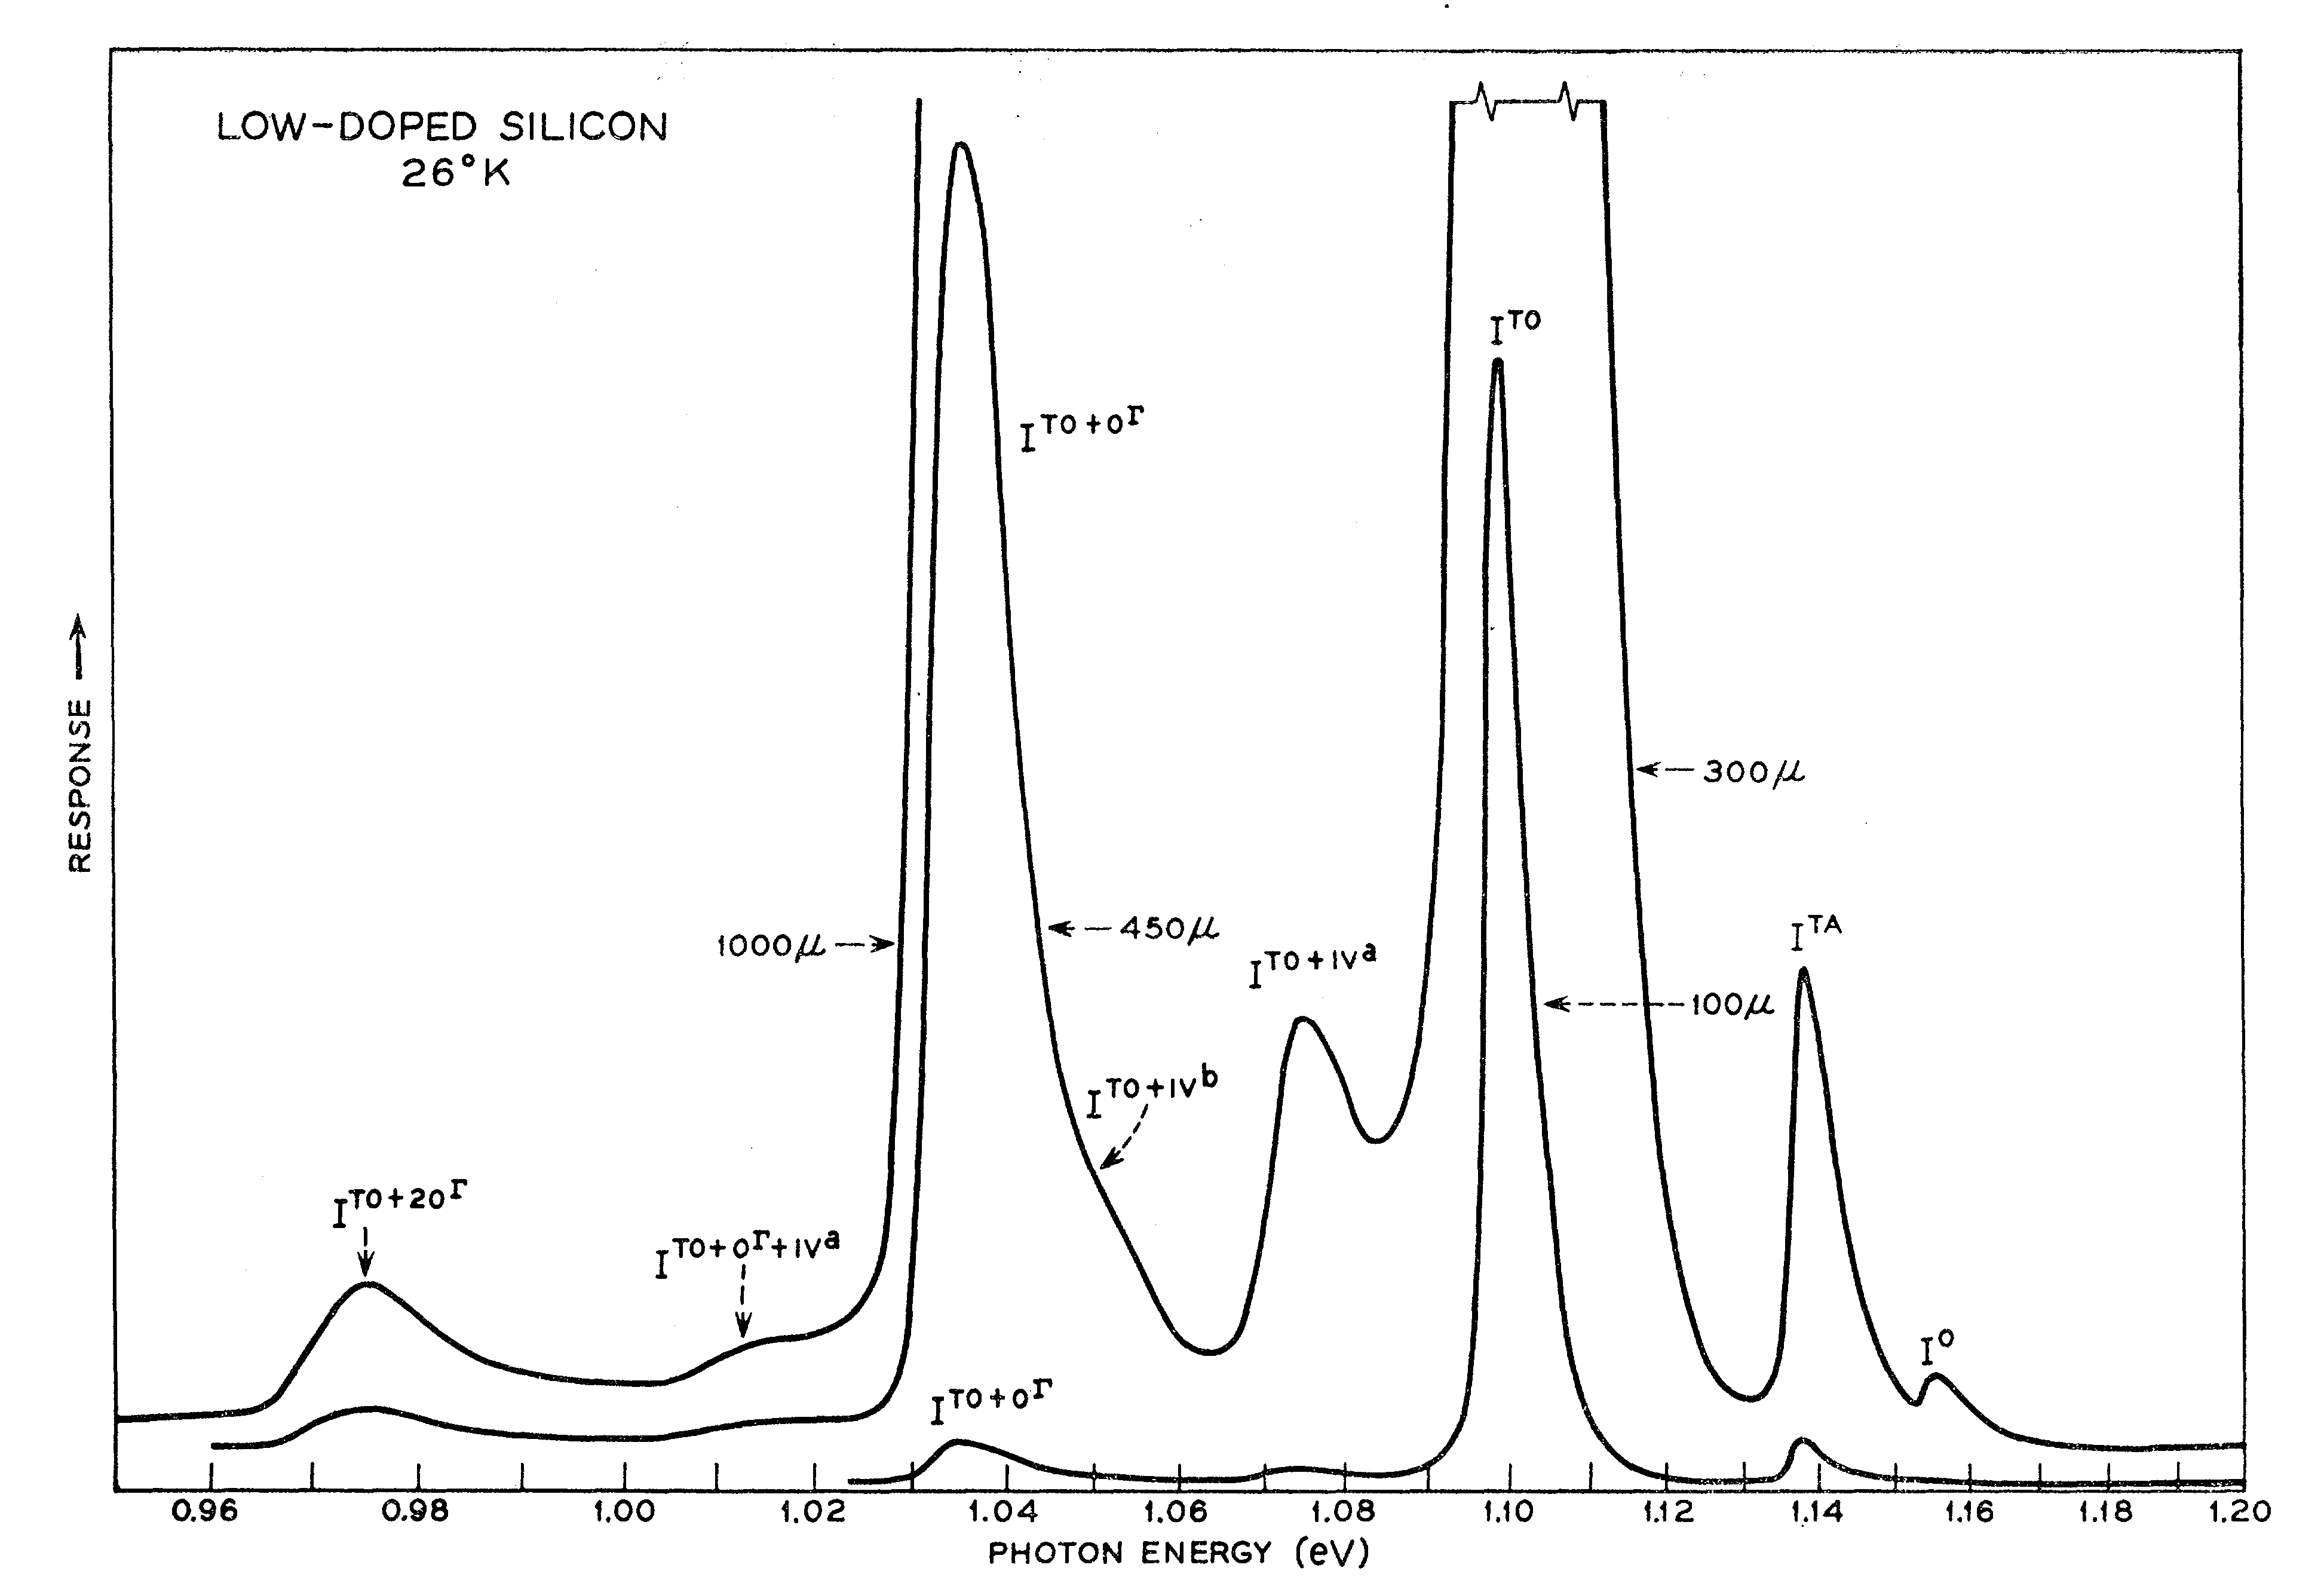
\includegraphics[width=15cm]{n-type_Si_spectra_dean67}
\caption{Intrinsic/low doped ($2\cdot10^{14}cm^{-3}$ P atoms) Si PL from \cite{dean67}}%
\label{fig:SiPL}%
\end{figure}

\begin{figure}
\centering
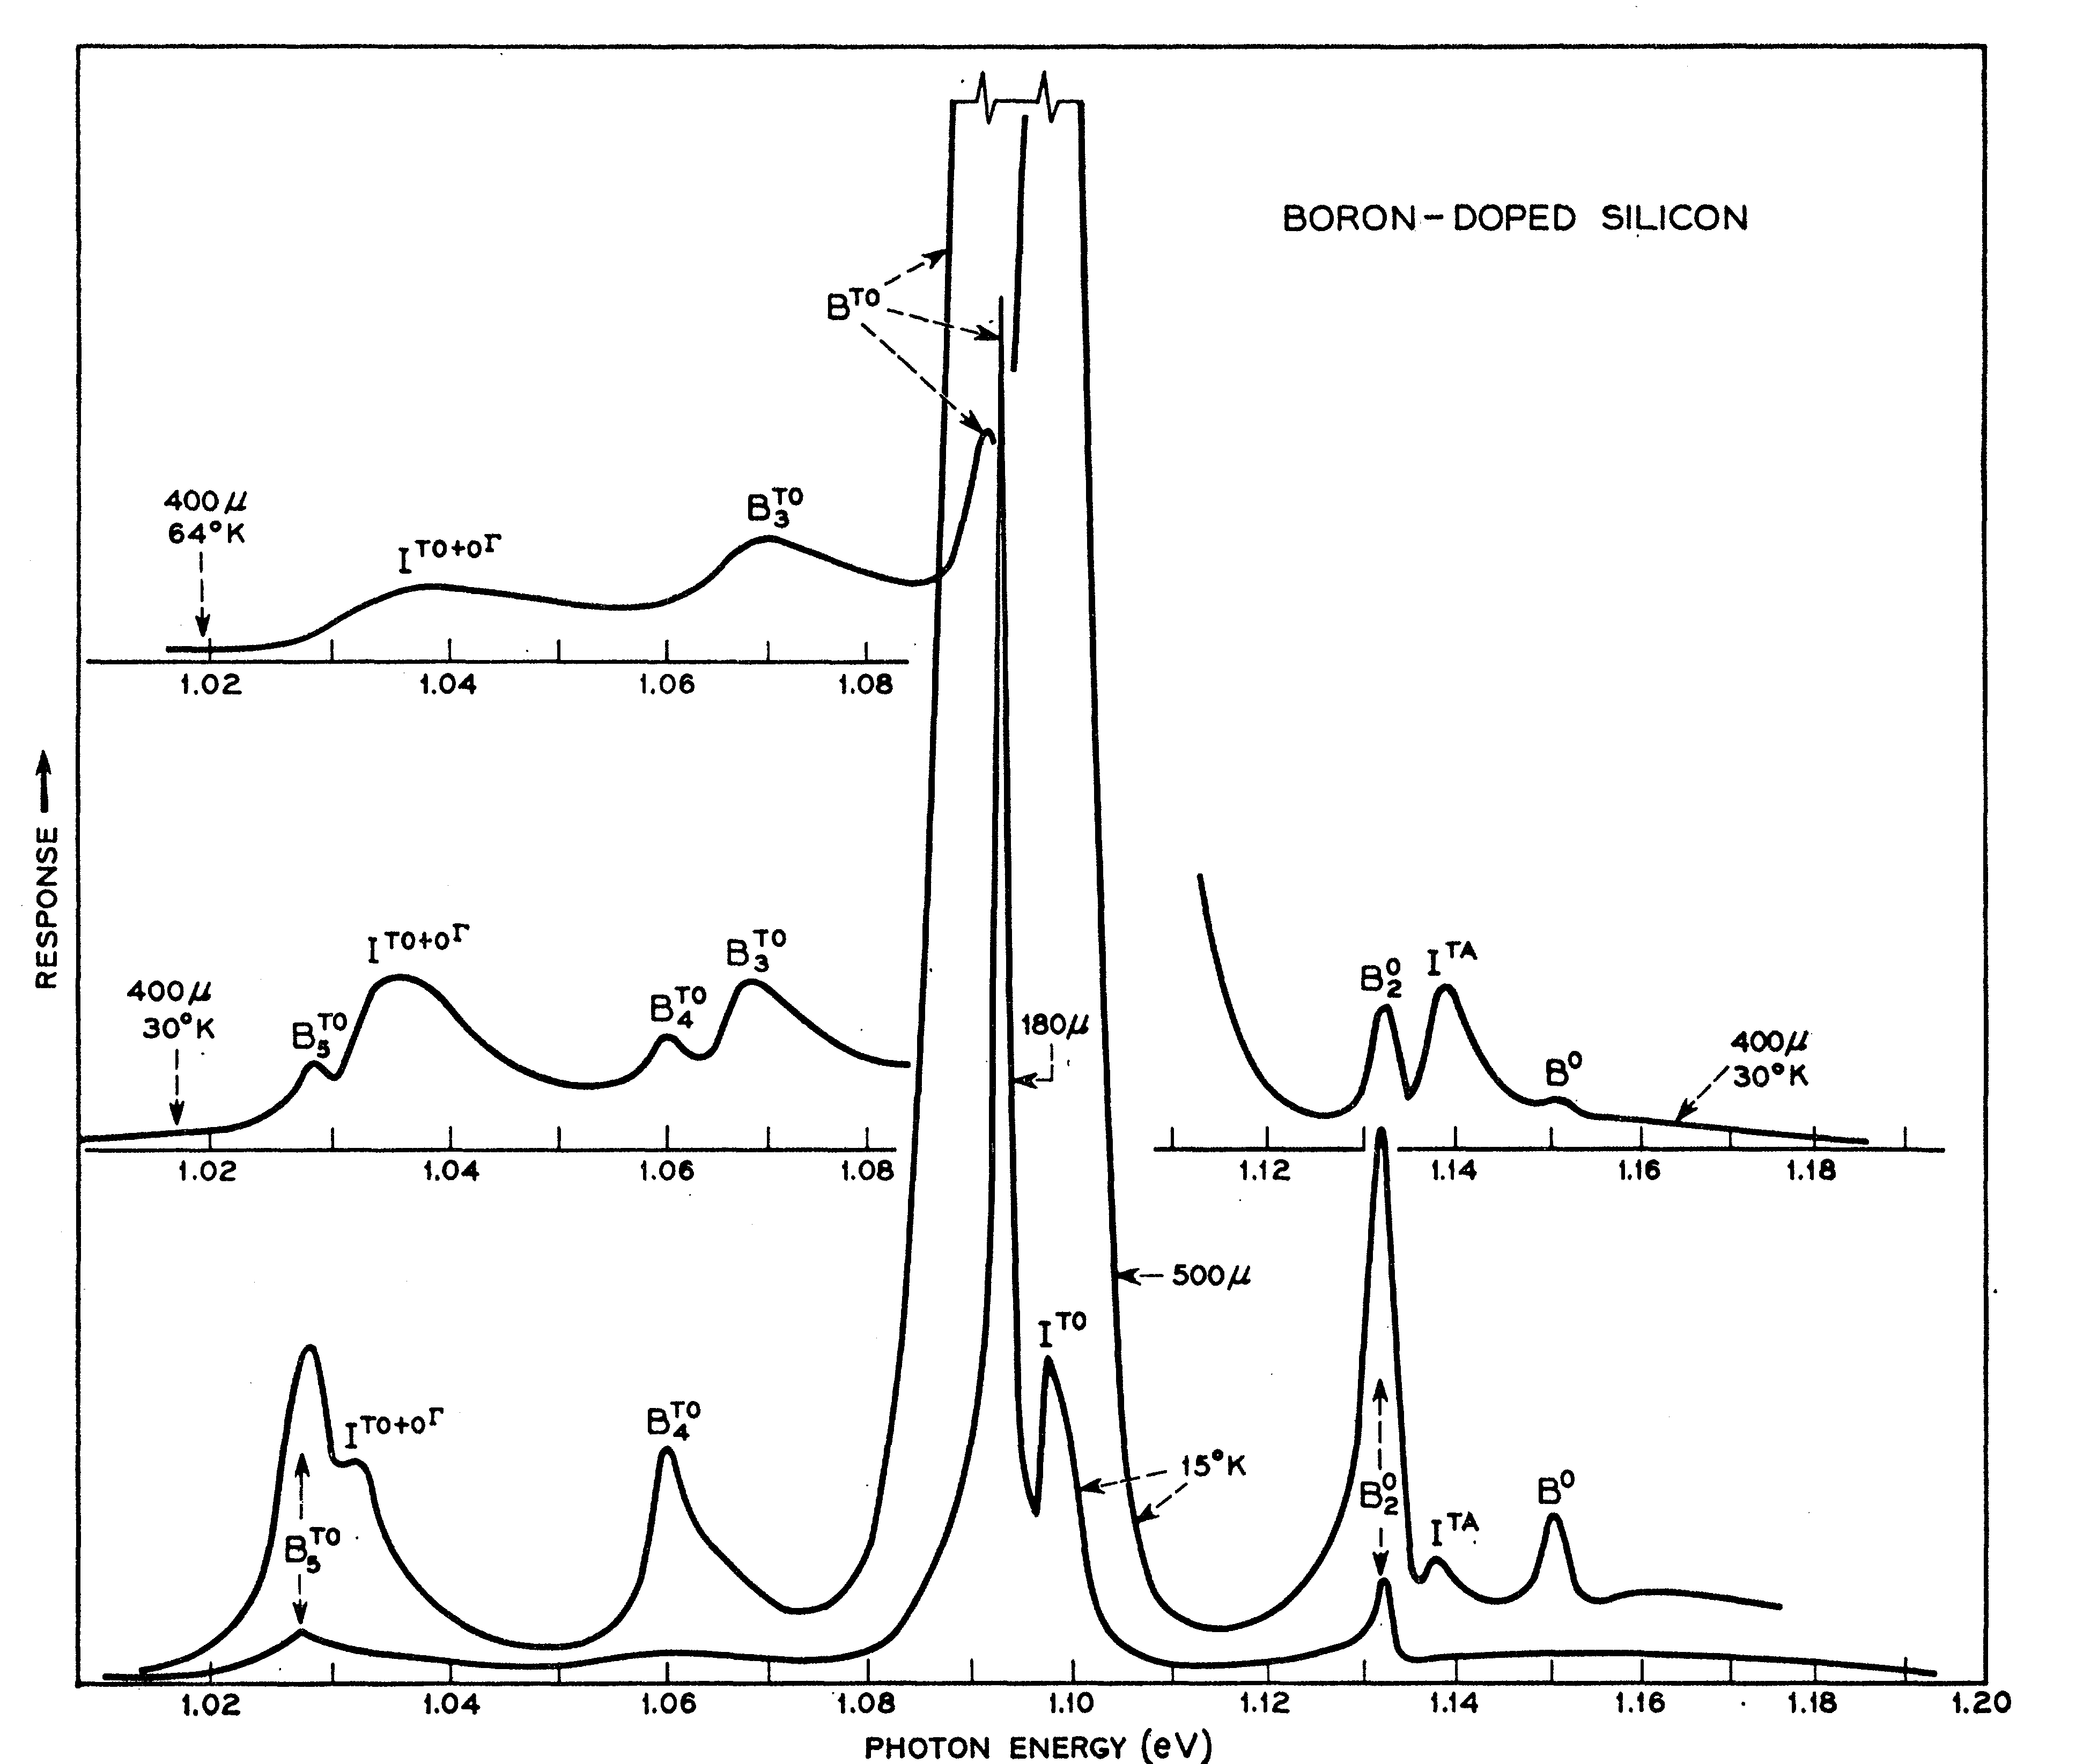
\includegraphics[width=15cm]{boron_Si_spectra_dean67}
\caption{Boron doped ($6\cdot10^{16}cm^{-3}$) Si PL specter from \cite{dean67}}%
\label{fig:boronSiPL}%
\end{figure}

\begin{figure}
\centering
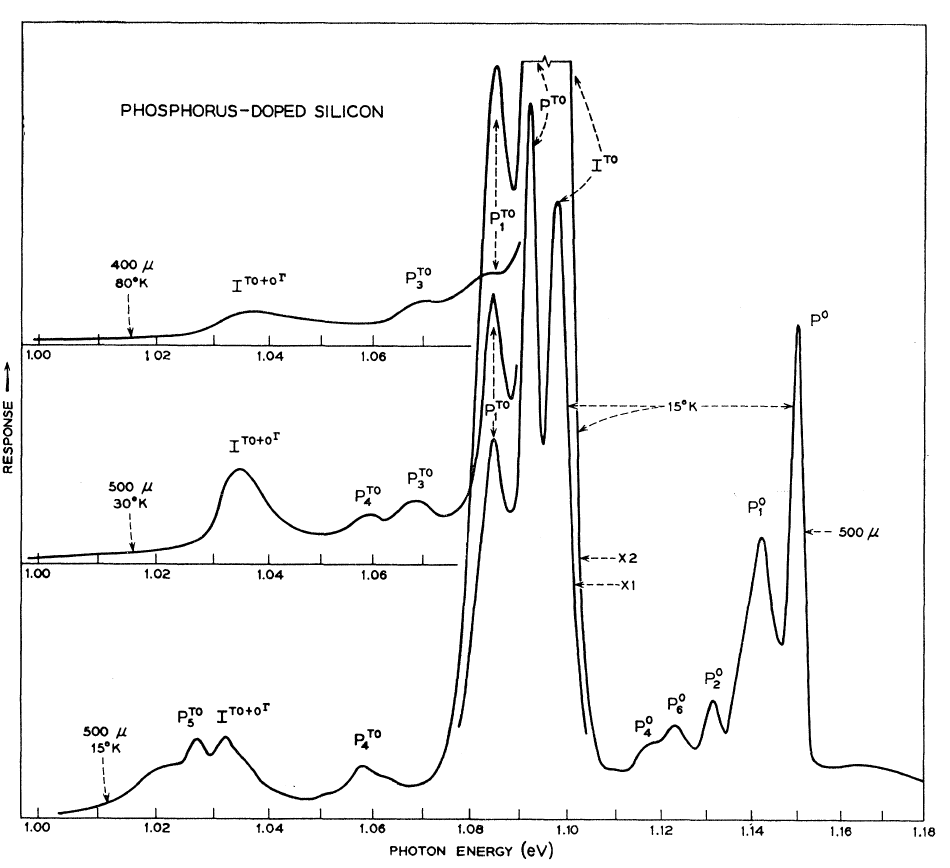
\includegraphics[width=15cm]{P_Si_spectra_dean67}
\caption{Phosphorus doped ($8\cdot10^{16}cm^{-3}$) Si PL specter from \cite{dean67}}%
\label{fig:PSiPL}%
\end{figure}


\begin{figure}
\centering
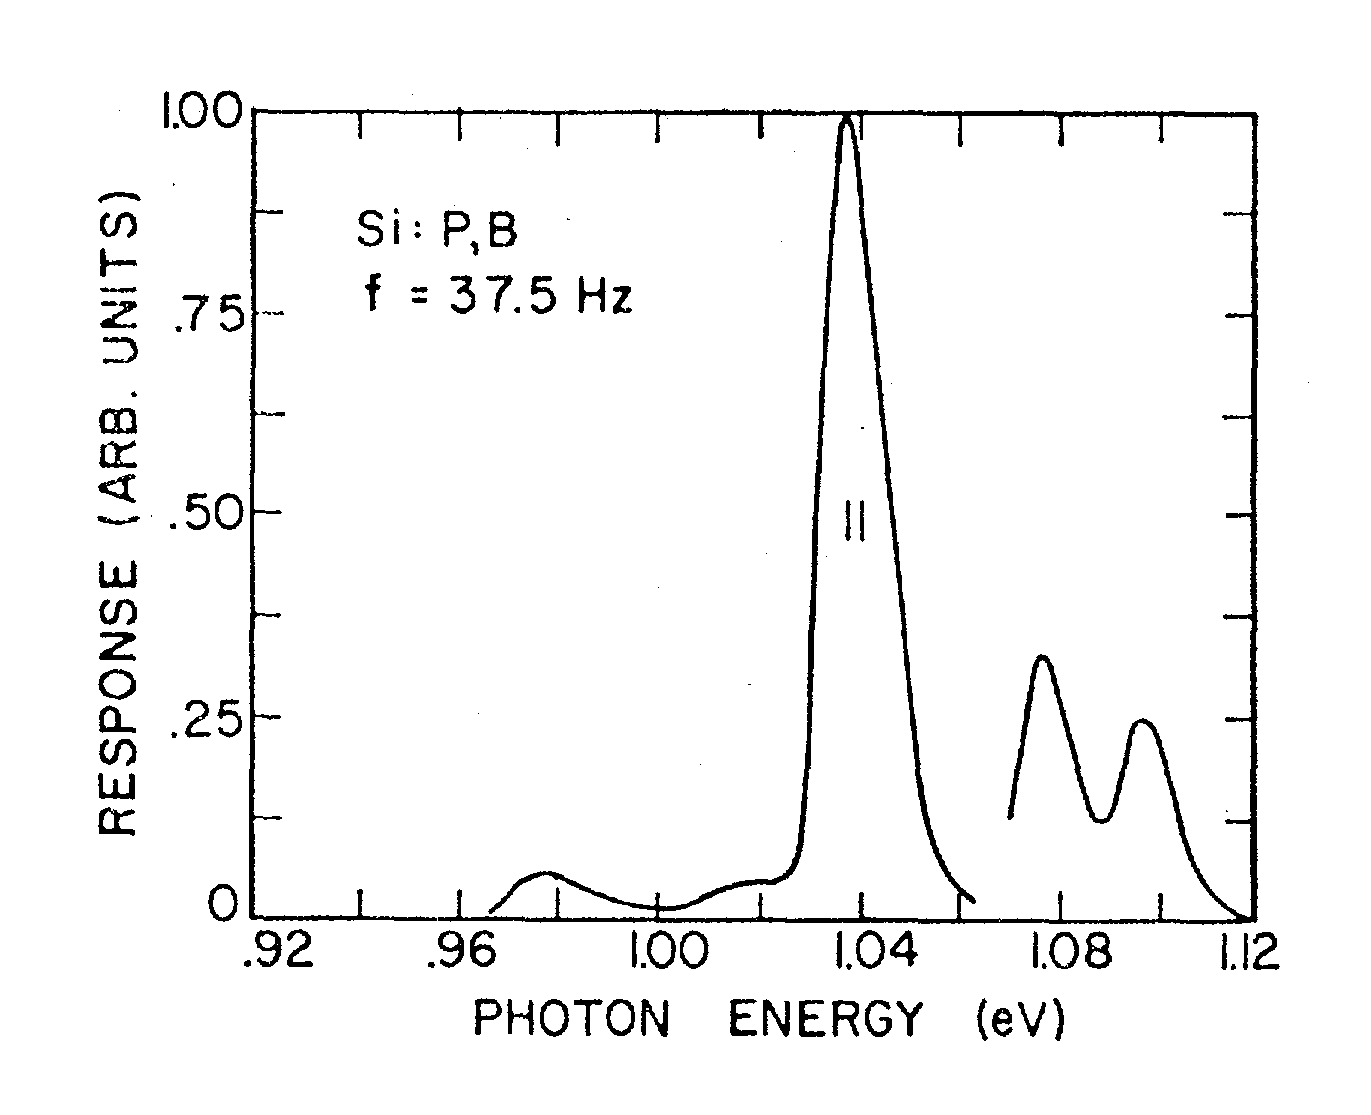
\includegraphics[width=15cm]{BP_luminescence}
\caption{Boron ($3\cdot10^{16}cm^{-3}$) and phosphorus ($6\cdot10^{16}cm^{-3}$) doped Si PL specter from \cite{enck69} at 4.2~K}%
\label{fig:BPSiPL}%
\end{figure}



\begin{figure}
\centering
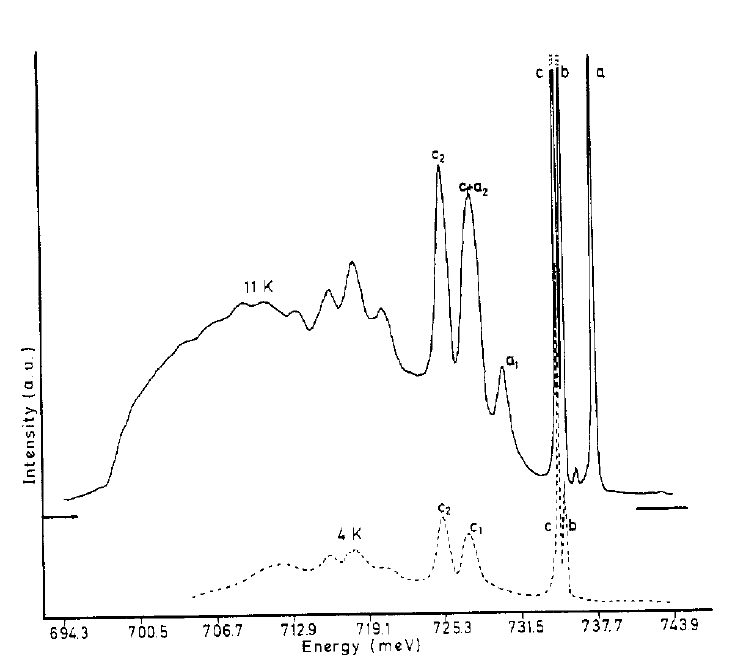
\includegraphics[width=15cm]{iron_diffused_Si_spectra}
\caption{Iron diffused Si sample at two different temperatures from \cite{calao88}}%
\label{fig:FeSiPL}%
\end{figure}


\begin{figure}
\centering
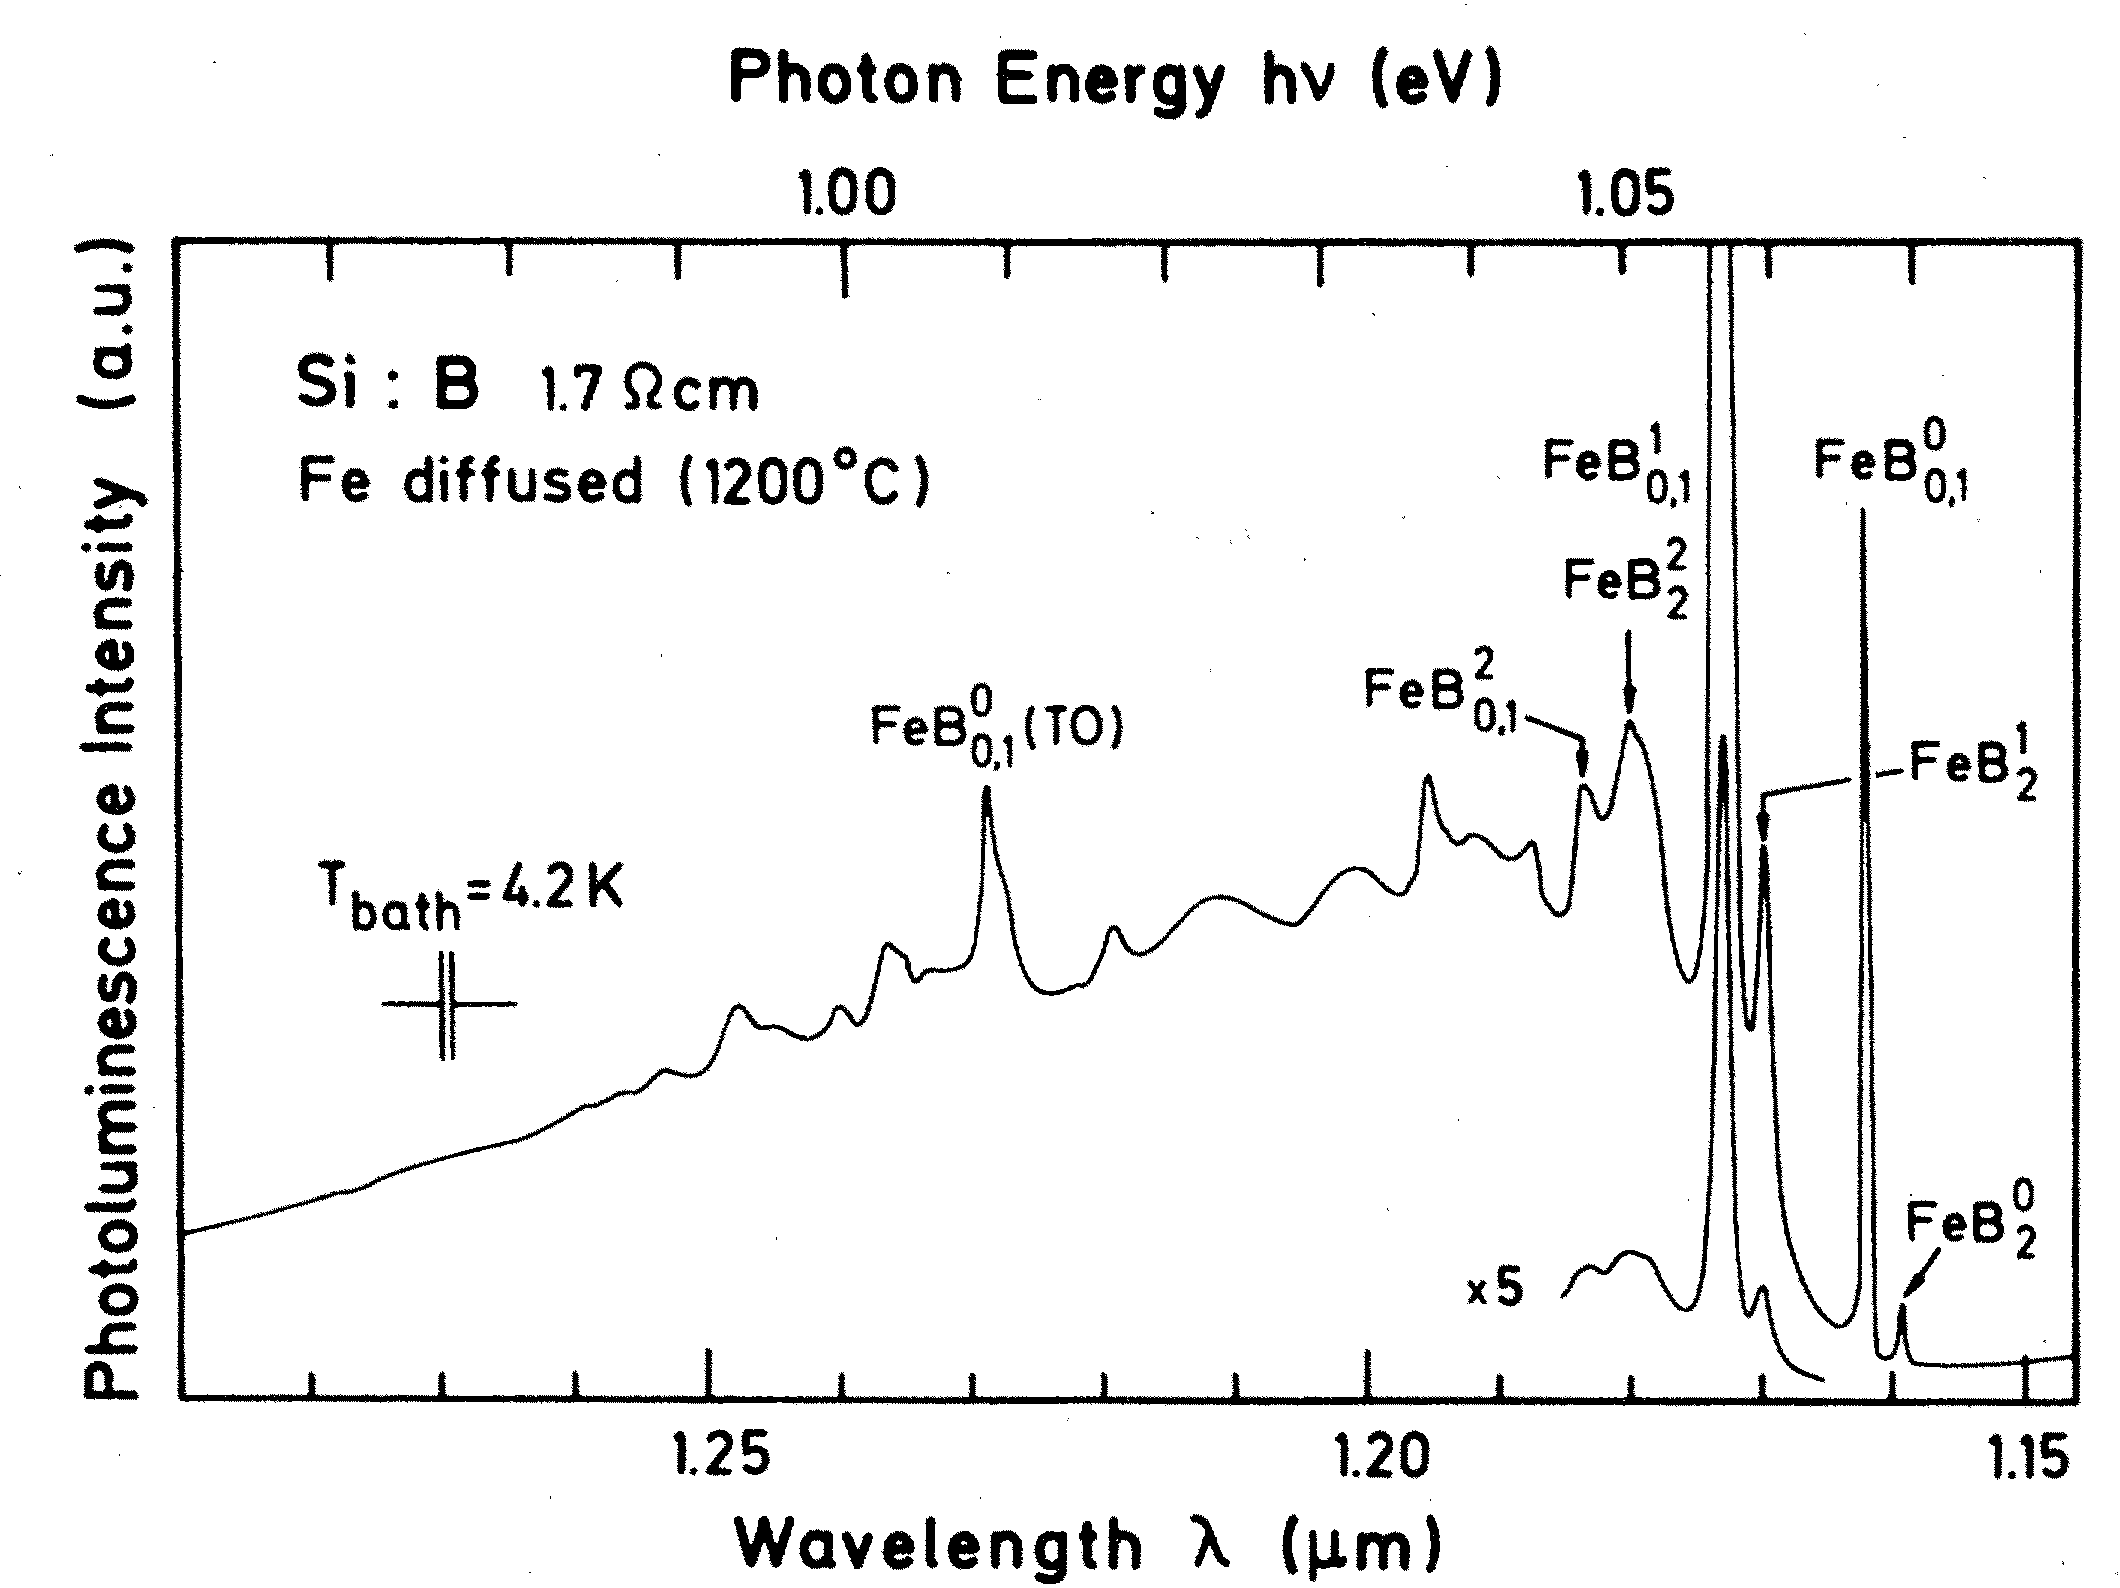
\includegraphics[width=15cm]{iron_diffused_boron_doped_Si_spectra}
\caption{Iron diffused boron doped Si sample from \cite{mohring83}}%
\label{fig:FeBSiPL}%
\end{figure}

\begin{figure}
\centering
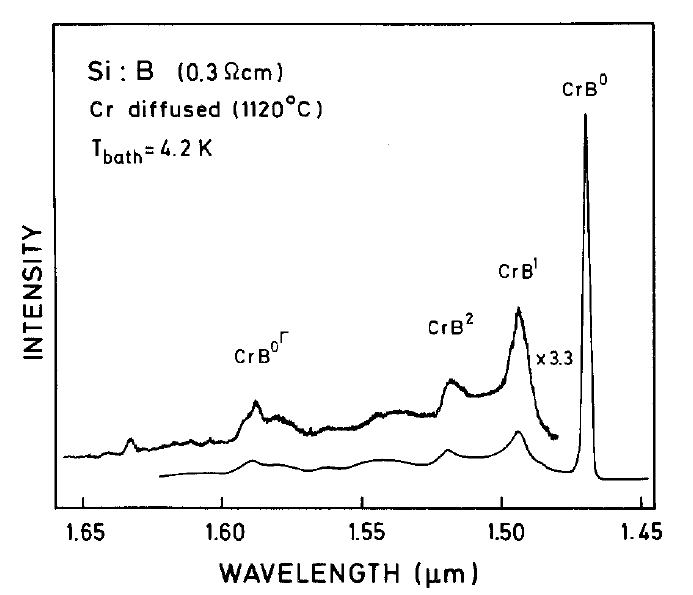
\includegraphics[width=15cm]{CrB_Si_spectra}
\caption{Chromium diffused Boron doped Si sample from \cite{conzelmann83}}%
\label{fig:CrBSiPL}%
\end{figure}


\begin{figure}%
\centering
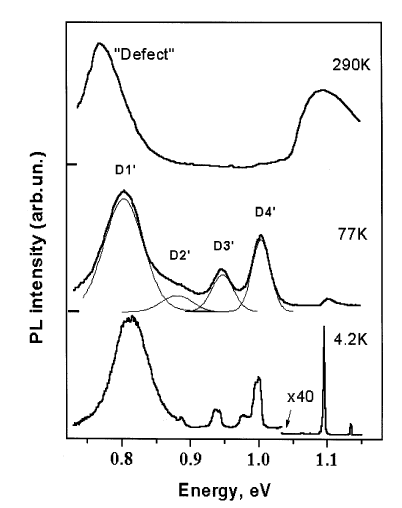
\includegraphics[width=10cm]{Dislocation_spectra}%
\caption[Dislocation lines from \cite{tarasov01}]{Dislocation related luminescence from mc-Si at different temperatures. The spectrum at 77 K is deconvolution numerical to resolve four individual Gaussian peaks. From \cite{tarasov01}.}%
\label{fig:Dislocation_spectra}%
\end{figure}


\begin{figure}%
\centering
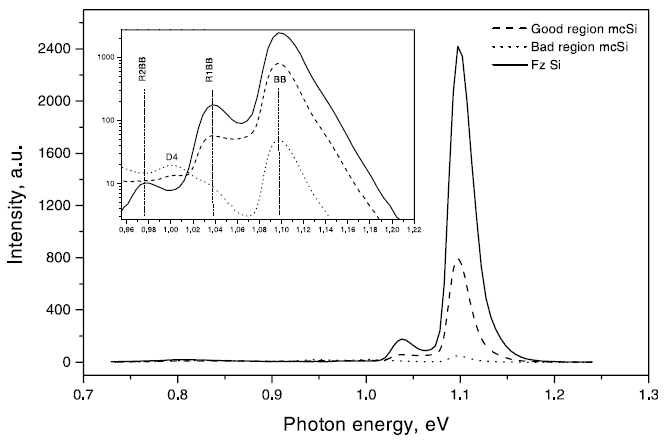
\includegraphics[width=10cm]{R1BB_plot}%
\caption[R1BB plot from \cite{arguirov03}]{Comparison of the spectra in high and low quality regions of mc-Si with FZ-Si from \cite{arguirov03}}%
\label{fig:R1BB}%
\end{figure}



\addtolength{\hoffset}{+1.5cm}
\begin{center}
\begin{sidewaystable}%
\small \begin{tabular}{|c|c|m{3cm}|m{4cm}|m{4cm}|m{2cm}|}

% Header for first page
%\hline 
%\multicolumn{1}{|c|}{\textbf{Ref.}} & 
%\multicolumn{1}{c|}{\textbf{Sample type}} & 
%\multicolumn{1}{c|}{\textbf{Excitation process}} & 
%\multicolumn{1}{c|}{\textbf{Area}} & 
%\multicolumn{1}{c|}{\textbf{Surface process}} & 
%\multicolumn{1}{c|}{\textbf{Doping}} \\ \hline
%\endfirsthead

% Header for page 2 3 4 etc.
%\multicolumn{6}{c}{{\bfseries \tablename\ \thetable{} -- continued from previous page}} \\
%\hline 
%\multicolumn{1}{|c|}{\textbf{Ref.}} & 
%\multicolumn{1}{c|}{\textbf{Sample type}} & 
%\multicolumn{1}{c|}{\textbf{Excitation process}} & 
%\multicolumn{1}{c|}{\textbf{Area}} & 
%\multicolumn{1}{c|}{\textbf{Processing}} & 
%\multicolumn{1}{c|}{\textbf{Doping}} \\ \hline\endhead

% Table footer on first pages
%\hline \multicolumn{6}{|r|}{{Continued on next page}} \\ \hline
%\endfoot

% Table footer on last page
%\endlastfoot
\hline
\textbf{Ref.} & \textbf{Sample type} & \textbf{Excitation process} & \textbf{Area} & \textbf{Processing} & \textbf{Doping} \\ \hline

\cite{sugimoto07} & mc-Si & 532nm Nd:YVO$_4$ & $0.1mW/10$ $�$m diameter & Sawing damage etched by HNO$_3$/HF & B-doped \\ \hline
\cite{tajima95} & Cz-Si & Kr ion laser 647nm & 10 \micro m &  & Undoped \\ \hline
\cite{drozdov76} & Cz-Si & Xenon lamp & 50mW on 3mm modulated at 9Hz & deformed by bending at 850$^\circ$ C & undoped, weak n and p \\ \hline
\cite{tarasov00} & mc-Si & 800nm AlGaAs laser & Pulsed 300mW / 3mm &  & Block-casting technique for Baysix \\ \hline
\cite{tarasov01} & mc-Si & 800nm AlGaAs at 140mW & & Produced by EFG & \\ \hline
\cite{arguirov03} & mc-Si and FZ-Si & Ar ion 514nm at 300mW & 100\micro m & Produced by EFG & boron doped $10^15cm^-1$ \\ \hline
\cite{sauer85} & FZ-Si & Kr-ion 647nm, Ar-ion 415nm and Nd-YAG 1064nm &  & Deformed a 650$^\circ$ C and 850$^\circ$ C & residual $10^{12}$cm$^{-3}$ boron \\ \hline
\cite{inoue07} & mc-Si & Nd:YVO 532nm & 6mW, 10$�$m diameter & Slicing damage etched off by HNO$_3$/HF & boron doped \\ \hline
\cite{conzelmann83} & FZ-Si and CZ-Si & & 50mW laser & Etched with HNO$_3$/HF. Chromium diffused & boron doped \\ \hline
\cite{mohring83} & FZ-Si & Ar$+$ 514nm & 500mW & Fe diffused & boron doped \\ \hline
\cite{calao88} & FZ-Si & Argon laser & & Fe diffusion & undoped \\ \hline
\cite{weber82} & & Ar$^+$ 514nm at 1.5W & & & Cu doped \\ \hline
\cite{weronek91} & FZ-Si & Ar$^+$ 514nm & & Heated above a Bunsen burner & Doped with Cu and/or Fe \\ \hline
\cite{binetti08} & mc-Si & & 6W/cm$^2$ & Polished by HNO$_3$/HF & Undoped \\ \hline
\cite{dean67} & CZ-Si & 200W mercury arc ~2.5eV & & & Undoped and doped \\ \hline
\cite{drozdov03} &  & Ar$^+$ or Kr$^+$ laser 0.6W & 0.8mm diameter & Dislocations by bending at ~700$^ \circ$C & phosphorus doped \\ \hline

\end{tabular}

\caption{Sample types and procedures}
\label{tab:sample_types}

\end{sidewaystable}
\end{center}


